% Compile with: pdflatex relations_after_the_fact.tex
% Two beamer slides illustrating:
%   1) ConceptGraphs' post-hoc relation inference
%   2) Why pure embedding-only retrieval fails at relational composition
\documentclass[aspectratio=169]{beamer}

\usetheme{default}
\usecolortheme{seahorse}
\setbeamertemplate{navigation symbols}{}
\setbeamertemplate{footline}{}

\usepackage{tikz}
\usetikzlibrary{arrows.meta, positioning, shapes.geometric, fit, backgrounds, decorations.pathreplacing}

\definecolor{farmblue}{RGB}{37,99,235}
\definecolor{farmgreen}{RGB}{22,163,74}
\definecolor{farmred}{RGB}{220,38,38}
\definecolor{farmgray}{RGB}{107,114,128}
\definecolor{farmbg}{RGB}{243,244,246}

\title{Relations After the Fact}
\subtitle{...and where pure embeddings fall short}

\begin{document}

% ---------------------------------------------------------------
% Slide 1: ConceptGraphs — relations inferred after mapping
% ---------------------------------------------------------------
\begin{frame}{Relations After the Fact}
\footnotesize
ConceptGraphs (Gu et al., 2024): build the open-vocabulary object set \emph{first},
then prompt an LLM \emph{after mapping} to infer relational edges from captions
and positions --- no hand-coded relation logic, the LLM decides what's ``on'' what.

\vspace{0.4cm}
\centering
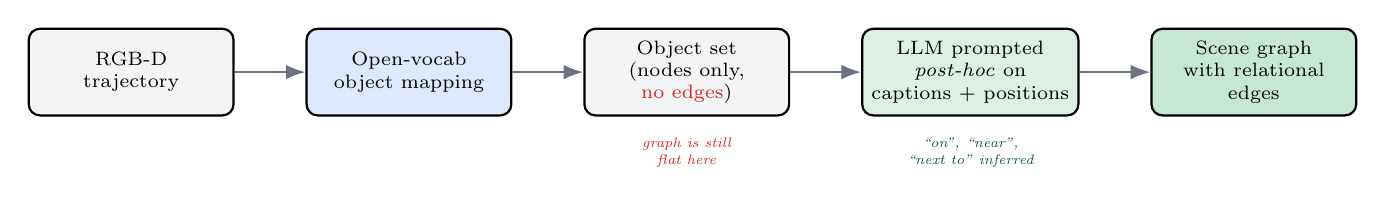
\begin{tikzpicture}[
    node distance=0.9cm,
    box/.style={draw, rounded corners, minimum height=1.1cm, minimum width=2.6cm,
                align=center, font=\scriptsize, fill=farmbg, thick},
    arr/.style={-{Latex[length=2.5mm]}, thick, farmgray}
  ]

  \node[box] (rgbd) {RGB-D\\trajectory};
  \node[box, right=of rgbd, fill=farmblue!15] (map) {Open-vocab\\object mapping};
  \node[box, right=of map] (objs) {Object set\\(nodes only,\\\textcolor{farmred}{no edges})};
  \node[box, right=of objs, fill=farmgreen!15] (llm) {LLM prompted\\\emph{post-hoc} on\\captions + positions};
  \node[box, right=of llm, fill=farmgreen!25] (graph) {Scene graph\\with relational\\edges};

  \draw[arr] (rgbd) -- (map);
  \draw[arr] (map) -- (objs);
  \draw[arr] (objs) -- (llm);
  \draw[arr] (llm) -- (graph);

  \node[below=0.15cm of objs, font=\tiny\itshape, farmred, align=center] {graph is still\\flat here};
  \node[below=0.15cm of llm, font=\tiny\itshape, farmgreen!60!black, align=center] {``on'', ``near'',\\``next to'' inferred};

\end{tikzpicture}

\vspace{0.3cm}
\scriptsize\textcolor{farmgray}{Mapping time and relation-inference time are decoupled: relations are a
\emph{second pass} over an already-built, relation-free object set.}
\end{frame}

% ---------------------------------------------------------------
% Slide 2: Embedding-only retrieval cannot compose relations
% ---------------------------------------------------------------
\begin{frame}{Where Pure Embeddings Fall Short}
\footnotesize
Query: \emph{``the glass on the table next to the laptop''} --- ranked purely by
similarity to \textbf{glass}, \textbf{table}, \textbf{laptop} \emph{separately}.

\vspace{0.25cm}
\centering
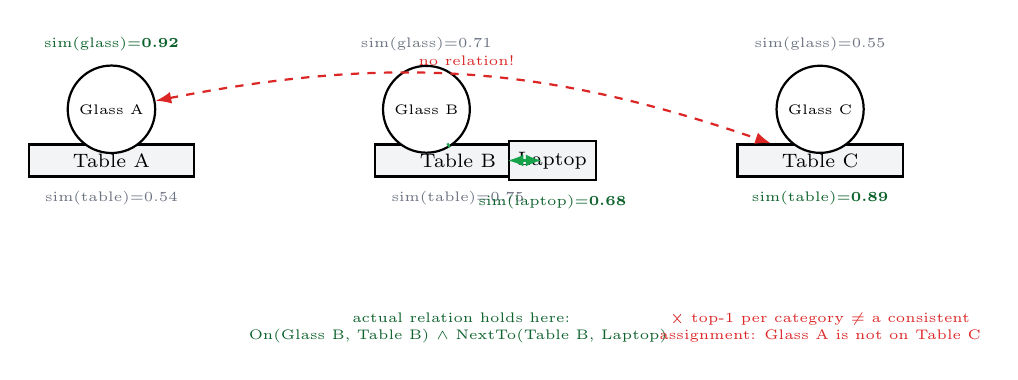
\begin{tikzpicture}[
    font=\scriptsize,
    tablestyle/.style={draw, thick, fill=farmbg, minimum width=2.1cm, minimum height=0.35cm},
    glassstyle/.style={draw, thick, circle, minimum size=0.55cm, fill=white},
    laptopstyle/.style={draw, thick, fill=farmbg, minimum width=1.1cm, minimum height=0.5cm}
  ]

  % --- Cluster A ---
  \node[tablestyle] (tableA) at (0,0) {Table A};
  \node[glassstyle] (glassA) at (0,0.65) {\tiny Glass A};
  \node[font=\tiny, farmgreen!60!black, above=0.05cm of glassA] {sim(glass)=\textbf{0.92}};
  \node[font=\tiny, farmgray, below=0.05cm of tableA] {sim(table)=0.54};

  % --- Cluster B (the actually-correct one) ---
  \node[tablestyle] (tableB) at (4.4,0) {Table B};
  \node[glassstyle] (glassB) at (4.0,0.65) {\tiny Glass B};
  \node[laptopstyle] (laptopB) at (5.6,0) {Laptop};
  \node[font=\tiny, farmgray, above=0.05cm of glassB] {sim(glass)=0.71};
  \node[font=\tiny, farmgray, below=0.05cm of tableB] {sim(table)=0.75};
  \node[font=\tiny, farmgreen!60!black, below=0.05cm of laptopB] {sim(laptop)=\textbf{0.68}};

  % --- Cluster C ---
  \node[tablestyle] (tableC) at (9.0,0) {Table C};
  \node[glassstyle] (glassC) at (9.0,0.65) {\tiny Glass C};
  \node[font=\tiny, farmgray, above=0.05cm of glassC] {sim(glass)=0.55};
  \node[font=\tiny, farmgreen!60!black, below=0.05cm of tableC] {sim(table)=\textbf{0.89}};

  % relations that actually hold (ground truth), drawn faint beneath cluster B
  \draw[farmgreen, thick] (glassB) -- (tableB);
  \draw[farmgreen, thick, {Latex[length=2mm]}-{Latex[length=2mm]}] (tableB) -- (laptopB);
  \node[font=\tiny, farmgreen!60!black, below=1.6cm of tableB, align=center]
    {\checkmark\ actual relation holds here:\\On(Glass B, Table B) $\wedge$ NextTo(Table B, Laptop)};

  % top-1-per-category picks by embedding alone: A, C, B -- physically inconsistent
  \draw[farmred, thick, dashed, {Latex[length=2mm]}-{Latex[length=2mm]}]
      (glassA) to[bend left=15] node[above, font=\tiny, farmred]{no relation!} (tableC);
  \node[font=\tiny, farmred, below=1.6cm of tableC, align=center]
    {\texttimes\ top-1 per category $\neq$ a consistent\\assignment: Glass A is not on Table C};

\end{tikzpicture}

\vspace{0.15cm}
\scriptsize Independently top-ranked objects (\textcolor{farmgreen!60!black}{bold scores}:
Glass~A, Table~C, Laptop~B) do not correspond to any single physical configuration ---
nothing enforces that the chosen glass is \textbf{on} the chosen table \textbf{and} that
table is \textbf{next to} the chosen laptop. This is the failure mode behind
\texttt{farm\_cabinet}: the right object is in the graph, correctly described, and still
doesn't surface.
\end{frame}

\end{document}
